% \documentclass[review]{elsarticle}
\documentclass[final,3p,times,onecolumn,sort&compress]{elsarticle}

\usepackage{lineno,hyperref}
\usepackage{listings}
\usepackage{subcaption}
\modulolinenumbers[2]

\usepackage{array}
\newenvironment{conditions}
  {\par\vspace{\abovedisplayskip}\noindent\begin{tabular}{>{$}l<{$} @{${}={}$} l}}
  {\end{tabular}\par\vspace{\belowdisplayskip}}
% \newcolumntype{R}{>{\raggedleft\arraybackslash}m{2cm}}


\usepackage{lmodern}
\usepackage[T1]{fontenc}
\usepackage{adjustbox}
\usepackage{booktabs}
\usepackage{multirow,makecell,rotating}
\usepackage[table]{xcolor}
\newcolumntype{s}{>{\columncolor[HTML]{E5E4E2}} c}
\newcolumntype{t}{>{\columncolor[HTML]{E5E4E2}} r}

\newcolumntype{R}[2]{%
    >{\adjustbox{angle=#1,lap=\width-(#2)}\bgroup}%
    l%
    <{\egroup}%
}
\newcommand*\rot{\multicolumn{1}{R{90}{1em}}}% no optional argument here, please!

\lstset{language=Python,
    basicstyle=\footnotesize\ttfamily,
    % commentstyle=\ttfamily\itshape\color{gray},
    stringstyle=\ttfamily,
    showstringspaces=false,
    breaklines=true,
    frameround=ffff,
    frame=single,
    % rulecolor=\color{black},https://www.overleaf.com/project/5e2b5d79fbc7fe0001583ea4
    tabsize=1,
    % keywordstyle=\color{red}\bfseries,
    columns=fullflexible,
    morekeywords={public, class}
    morecomment=[s]{"""}{"""},
}

\journal{ }

%% Elsevier bibliography styles
%% APA style
\bibliographystyle{model5-names}\biboptions{authoryear}

%%%%%%%%%%%%%%%%%%%%%%%

\begin{document}

\begin{frontmatter}

\title{Measuring inequalities in urban systems: An approach for evaluating the distribution of amenities and burdens}

% \author[1,4]{T M Logan\corref{mycorrespondingauthor}}
% \ead{tom.logan@canterbury.ac.nz}
% \author[1,4]{M J Anderson}
% \author[2]{T G Williams}
% \author[3,4]{L Conrow}

% \address[1]{Civil and Natural Resources Engineering, University of Canterbury, New Zealand}
% \address[2]{Industrial and Operations Engineering, University of Michigan, Ann Arbor, USA}
% \address[3]{Earth and Environment, University of Canterbury, New Zealand}
% \address[4]{The Cluster for Community and Urban Resilience, University of Canterbury, New Zealand}

\begin{abstract}
Current approaches for measuring inequality are insufficient or unsuitable for promoting and designing equitable built environments and urban systems.
In this paper, we demonstrate how a recently developed inequality measure---the Kolm-Pollak equally-distributed equivalent (EDE)---could be used to support decision making to foster equity in the built environment.
The EDE provides a measure of a distribution that is similar to the average (mean) but includes a penalty based on the inequality of that distribution.
The primary advantage of the Kolm-Pollak EDE is that it can be used to evaluate the inequality of both desirable quantities (e.g., amenities) and undesirable quantities (e.g., burdens).
This is essential in urban systems as inequities can manifest through, among other things, disparate access to opportunities like public amenities and unequal exposure to burdens, such as pollution and natural hazards.
Additionally, the Kolm-Pollak EDE can be calculated for different sociodemographic subgroups, enabling needs-based assessments to promote environmental justice.
Thus, the Kolm-Pollak EDE presents numerous opportunities for practitioners, policymakers, and researchers concerned with advancing equity.
We demonstrate the approach with a case study of grocery store access in ten cities across the USA and provide a Python package (\textit{inequalipy}) to enable others to use these inequality metrics.
\end{abstract}

\begin{keyword}
Equity $|$ Equality $|$ Environmental justice $|$ Urban planning $|$ Food desert 
\end{keyword}

\end{frontmatter}

\linenumbers

\section{Introduction}
The distribution of amenities and burdens within our communities will change as we adapt our cities to global change.
These required changes present an opportunity to both ensure people have acceptable access to opportunities and reduce their exposure to burdens, as well as to ensure the distributions of these are fair.
This fairness is critical for community trust and cohesion, which is a necessary condition for community sustainability and resilience \citep{Dempsey2011-og, Cutter2008-NJ, Logan2020-vj}.
Thus, there is a global and time-critical imperative to improve the distribution of resources and burdens within the built environment.
To deliver optimal and fair allocations, planners, policymakers, designers, and engineers need the ability to evaluate scenarios, through the lens of equity, in a substantive manner.

How we design our communities and react to environmental change influences how burdens and resources are distributed between residents \citep{Marino2012-lq,Wilson2008-yk, Calvin2017-ja}.
These burdens include exposure to air pollution \citep{Maguire2011-fi, Sheriff2020-ge}, natural hazards \citep{Burby2000-qe, Saunders2007-of}, commute time \citep{Frumkin2004-yi}, and chronic diseases \citep{Lopez2006-jb}.
Resources, many of which ameliorate some of these burdens, include trees, supermarkets, schools, health care, and green space \citep{Schwarz2015-fs, Logan2019-fr, Nesbitt2019-sk, Pacione1989-ui, Apparicio2007-di, Whitehead2019-tf}.
For example, access to healthy food improves people's diets, which improves their health \citep{Garcia2020-xt, Kolak2018-az}.
Parks and green spaces mitigate flooding, heat, erosion, and air pollution, while providing opportunities for recreation, improved mental health, and forging social capital \citep{Dempsey2011-og, Astell-Burt2013-og,Kazmierczak2011-ot, Norton2015-vv}.
Unfortunately, empirical evidence consistently reveals that these burdens and resources are not equally distributed among people;
globally disadvantaged and underprivileged people are systematically exposed to larger environmental burdens and have worse access to beneficial resources \citep{Fussel2010-te, Bulkeley2014-so}.
Future development and changes to urban form threaten to increase these disparities \citep{Gusdorf2008-bm, Calvin2017-ja}.

Fairness, and what it constitutes, is characterized by the concepts of equality, equity, and environmental justice \citep{Talen1998-mk, Low2013-yx, Rigolon2019-zr, Lopez2011-cc}.
Equality is where everyone receives the same amount of a resource, whereas equity is where the resource is distributed based on people's needs \citep{Talen1998-mk, Lucy1981-xr}.
For example, \cite{Rumley2014-pu} provided the anecdote that giving two children each an apple achieves equality; however, this is not equitable if one child has not eaten in three days. 
In turn, environmental justice---the notion that everyone has the right to a healthy environment \citep{Lopez2011-cc}---is achieved through equity in distributional, interactional, and procedural justice \citep{Low2013-yx}.
Distributional justice is influenced by where we locate resources and guide residential development.
How we create spaces influences interactional justice, as approaches such as mixed-use design encourage a diversity of users and enable people to interact safely \citep{Jacobs1961-po}.
Whether communities are empowered and engaged during the decision-making process influences procedural justice \citep{Low2013-yx, Rigolon2019-zr}.

Therefore, to promote environmental justice, we require a substantive measure of a distribution that penalizes for inequality and can also be used to guide the decision-making process by evaluating policies and interventions.
In urban contexts, such an equality measure needs to both consider the equality of the subgroups (separability) and represent the scale and location of the distribution (cf. a relative index). 
Some degree of inequality is expected in urban contexts because some people will inherently live closer to a resource than others \citep{Dadashpoor2016-ar, Nesbitt2019-sk}, while at the same time, equity may necessitate inequality when populations have differential needs. 
Measuring equality is a critical precursor to assessing equity because equity depends on the state of inequality. 
Some groups within our communities simply need more of some resources than others. 
For example, youth need access to schools, while older people need better access to health care \citep{Syed2013-aj}. 
In practice, analyses based on equity often begin with an assessment of equality, which is then coupled with an evaluation of need, based on socioeconomic information \citep{Talen1998-mk, Whitehead2019-tf, Schwarz2015-fs, Harlan2006-ap}.
Understanding, visualizing, and quantifying how resources are allocated and the fairness of distributions is a significant tool for supporting decision-makers to incentivize development to ensure the future changes are both widely beneficial and fair. 

Existing measures of inequality, however, have had major limitations that restrict their use in urban contexts. 
Fortunately, those limitations have been addressed by a recently proposed measure of equality---the Kolm-Pollak method \citep{Sheriff2020-ge}.
The objective of this paper is to:
\begin{enumerate}
    \item Describe a quantitative approach for measuring inequality that is suitable for urban systems. That is, it
    \begin{itemize}
        \item can evaluate the distribution of both desirable and undesirable quantities
        \item can consider separate socioeconomic groups to analyze and compare equity with differential impacts among those subgroups
        \item is suitable for comparing interventions or scenarios based on overall benefit and impacts on equity.
    \end{itemize}
    \item Demonstrate this approach with a case study of access to grocery stores.
\end{enumerate}

The remainder of this paper is structured as follows. In \autoref{sec:measuring}, we describe the existing approaches for measuring equality in urban systems. 
We then outline the Kolm-Pollak measure in section \ref{sec:method} and summarize the desirable criteria for an inequality measure in urban systems in section \ref{sec:criteria}.
We then demonstrate the Kolm-Pollak's application in section \ref{sec:case} through three examples in the context of food access in the USA:
access to grocery stores in ten cities;
subgroup-level analysis to evaluate equity in this access; and
changes in supermarket access in Chicago since 2007.
Finally, we provide some concluding thoughts in section \ref{sec:discussion}.

\section{Background: Measuring equality in urban systems}
\label{sec:measuring}
The built environment and urban form significantly affect both distributional and interactional justice. 
In these contexts, equity has been assessed using regression and correlation analysis, equity mapping, cluster analysis, and summary statistics.

Regression and correlation approaches typically assess whether there are consistent disparities in access or distribution based on any of the socioeconomic or demographic factors considered, as applied in studies such as \cite{Schwarz2015-fs, Nesbitt2019-sk, Kim2016-mc, Williams2020-greenspace, Apparicio2007-di}.
Map-based visualizations, such as equity mapping \citep{Talen1998-fl, Wolch2005-wz}, identify specific regions lacking in or over-exposed to the quantity in question.
As an extension of mapping, spatial clustering and spatial autocorrelation approaches are used to assess the relationship between some quantity’s spatial distribution and other variables, often socioeconomic or demographic, in neighboring areas \citep{Talen1997-gl, Smoyer-Tomic2004-eh,Garcia2020-xt}.
\textbf{While the Mann-Whitney U test can be applied to compare values in neighboring geographic areas when data lack normality and independence \citep{Nicholls2001-pf}, the principal approach in examining spatial patterns of distributed values is \cite{Anselin1995-fh}'s Local Indicators of Spatial Autocorrelation (LISA). 
Maps, or the mapped results of LISA, are essential tools that enable decision-makers and residents to understand the geographic arrangement of resources and allow them to visualize how decisions influence disparities \citep{Talen1998-fl}.
These approaches highlight relationships between various factors and spatial arrangements that may influence inequity, aiming to determine where significant patterns of need intersect with significant patterns of access. 
Mapping LISA results allows clusters (e.g., high values with high neighboring values) and outliers (e.g., high values with low neighboring values) to be interpreted within the context of the topic under study, and their primary utility is in identifying those locations. 
LISA are a decomposition of global spatial autocorrelation statistics, where meaningful patterns can be obscured within the global measure of overall spatial autocorrelation \citep{Talen1998-mk}. 
The LISA value for each area measures its contribution to the global counterpart, though neither is necessarily an evaluation of the overall level of inequity in the study area.
}

Quantitative summary statistics describe the statistical distribution, and therefore overall inequality.
% , however, these existing measures can obscure disparities or might be unsuitable in planning contexts \citep{Kolak2018-az,Logan2019-fr}.
Quantitative summary measures can complement map-based approaches, as they are necessary to support analysis such as ranking interventions, ranking cities for allocating assistance, or for optimization in a manner that visualizations are unable to support.
Summary statistics are generally categorized as a measure of a distribution’s dispersion (aka. the spread or variation), central location (i.e., its approximate value), or a measure of position (e.g., the quantiles or the percentage of people within some threshold value).
For example, simple summary statistics for a distribution’s central location include the mean, median, and well-known summary statistics for dispersion include standard deviation, variance, and range.
Commonly used measures of equality tend to be drawn from these dispersion statistics, most notably the Gini coefficient, which is a relative measure of the difference between the current distribution and the state of everyone receiving the exact same value (“perfect” equality).
The coefficient of variation (CV) is another measure of dispersion, as it is the standard deviation normalized by the mean.
It was first used in an urban planning context to assess equality in accessing school locations \citep{Pacione1989-ui}. 

\begin{figure*}
    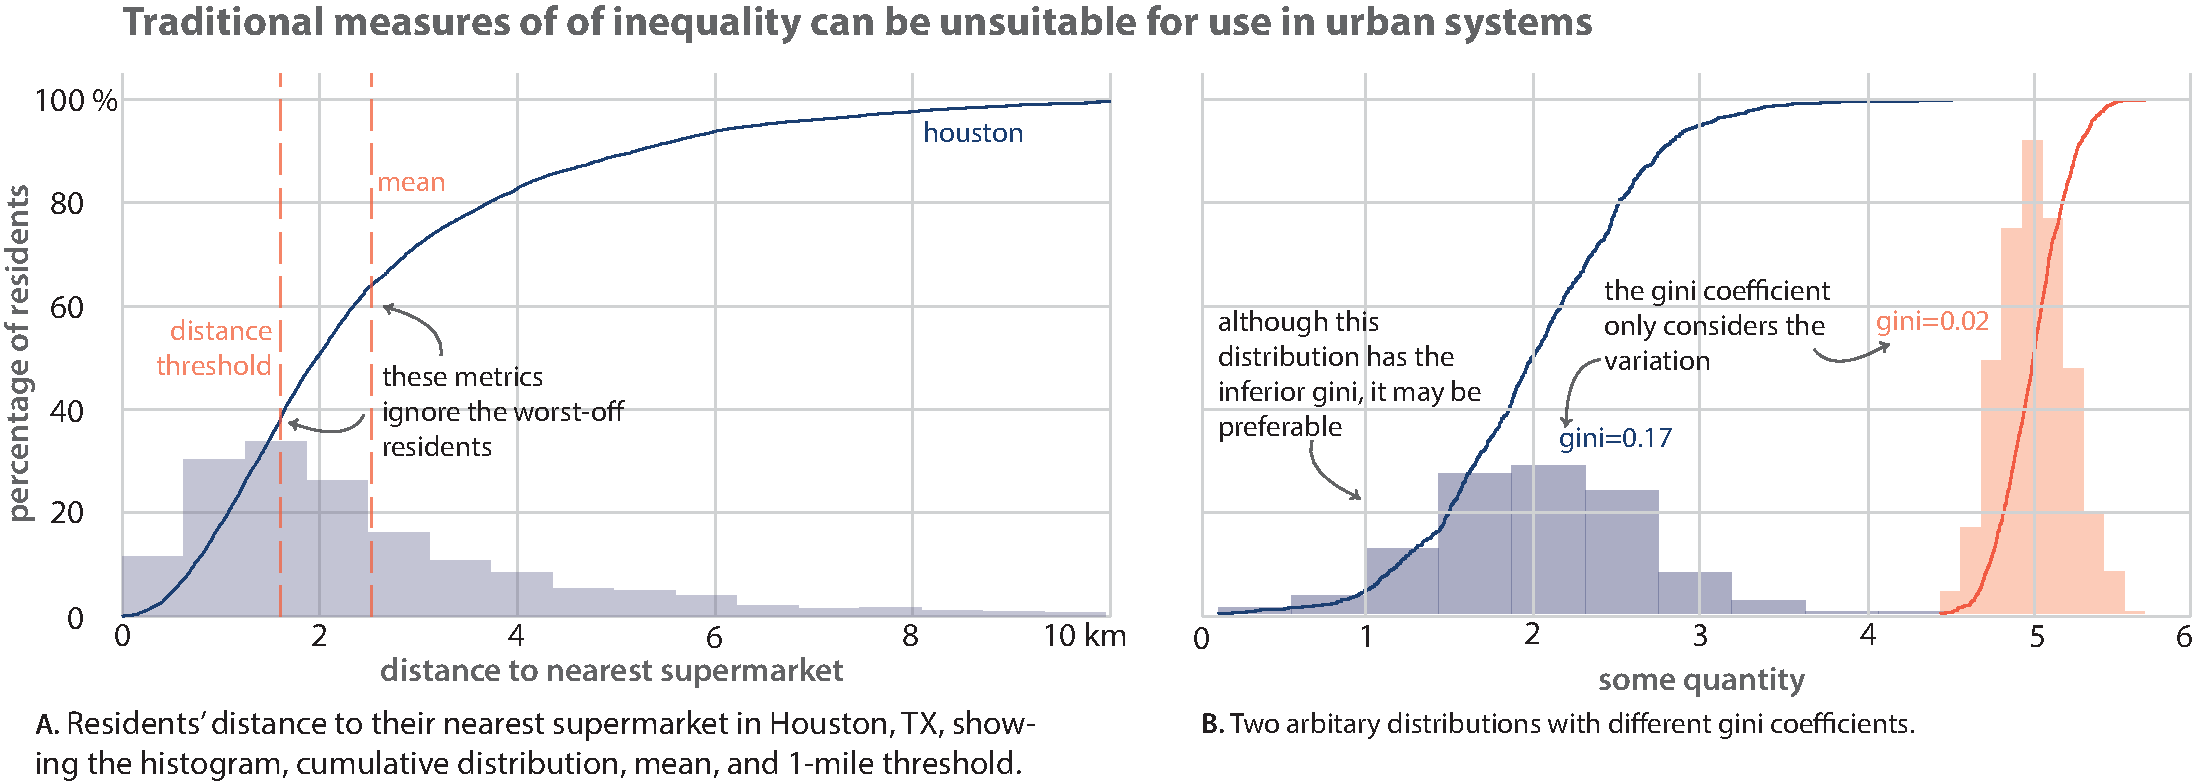
\includegraphics[width=0.9\linewidth]{report/fig/fig1v2.pdf} 
    \caption{Traditional measures of distributions are insufficient for representing inequality. 
    Figure 1A shows the residents' distance to their nearest grocery store in Houston, TX, showing the histogram and cumulative distribution, along with the mean and 1-mile threshold. 
    These measures cannot both describe the location (aka. central tendency of a distribution) as well as reflect the state of the individuals at the tail end of the distribution.
    Figure 1B shows how the Gini coefficient ignores the location and so can prefer unfavourable distributions.}
    \label{fig:current_metrics}
\end{figure*}

\textbf{Despite their widespread use and simplicity, summary statistics can be inappropriate in urban contexts as some do not reflect the severity of the worst-off individuals, are relative (scale independent) measures, and/or embody implicit assumptions concerning distributional justice. 
To demonstrate these limitations, consider the distance that Houston (Texas) residents live to their nearest grocery store (Figure \ref{fig:current_metrics}a). 
To begin with, measures of central location (e.g., the mean) or position (e.g., the percentage of people that live within some distance) can ignore the tail-end of the distribution: the worst-off individuals (Figure \ref{fig:current_metrics}a). 
Alternatively, measures of dispersion (e.g., standard deviation, Gini) are scale-independent, meaning that they are independent of the distance residents live from their nearest store (Figure \ref{fig:current_metrics}b).
Considering relative (scale independent) values may be useful when comparing the wealth distributions of countries with different GDPs, however, in urban contexts, the scale of a distribution matters if the focus is on what people experience. 
In such contexts, it is plausible that a less equal distribution may be more desirable in some instances.
One such instance is a hazard context: consider the situation (1) where everyone is equally majorly affected by an event, and contrast this with the situation (2) where some residents are not impacted but others are slightly affected.
Situation (2) is likely preferable, even though it is less equal.
An additional limitation of ‘positive’ measures (cf. normative measures) such as the Gini coefficient and CV is that they involve implicit assumptions about the desirability of transfers and the aversion to inequality \citep{Maguire2011-fi, Atkinson1970-mr, Adger1997-tu}.}
% Essentially, these statistical measures of dispersion do not prioritize improving the state of the ‘poorest’ individuals.
% are unsuitable or unsatisfactory for measuring equality as a desirable concept 

To address these limitations, \cite{Atkinson1970-mr} proposed using an equally-distributed equivalent (EDE).
This is a measure of the central location of a distribution, penalized for inequality based on a social welfare function.
An EDE represents the value that would, if everyone had that same value, provide the same level of welfare as the existing distribution.
An EDE is analogous to the risk premium or certainty equivalent from decision science and is, in practice, an alternative summary statistic for a distribution that captures both the location and the dispersion of a distribution.
Unlike ‘positive’ summary statistics, however, the EDE is based on a subjective parameter that represents aversion to inequality and is how welfare is determined.
The use of this parameter means that the value judgment regarding the importance of inequality shifts from being implicit, as it is for the Gini coefficient and coefficient of variation, to being explicit and user-defined.
While some people may be uncomfortable with the subjectivity of a user-defined parameter, the alternative measures (such as the Gini) each carry implicit value judgments as to the importance of and aversion to inequality.
\textbf{Instead, using an aversion parameter can accommodate different views concerning distributional justice and enables us to evaluate how sensitive the rank order of alternative interventions is to that aversion.}
That is, as \cite{Atkinson1970-mr} points out, any evaluation of inequality involves judgments relating to social welfare---a normative approach enables us to explore the effect of these judgments.

While Atkinson's approach has proven useful for evaluating the inequality of income, it is unsuitable for distributions of undesirable quantities \citep{Cox2012-lg, Sheriff2020-ge, Maguire2011-fi, Fann2011-hd} — a crucial question of planners.
Simply inverting an undesirable distribution to evaluate the equality of the complement (e.g., using $\frac{1}{x}$ instead of $x$) does not address this problem because the rank order (order of preference when comparing distributions) can change between the undesirable quantity and its complementary good \citep{Sheriff2020-ge, Cox2012-lg, Erreygers2009-is}.
This issue with the Atkinson EDE (and associated index) was recently addressed through adjustments to the Kolm-Pollak approach \citep{Sheriff2020-ge}. 
The Kolm-Pollak approach also uses an EDE, however, it is mathematically distinct from Atkinson’s. 
The important difference is that the Kolm-Pollak approach has been constructed to evaluate the distribution of both desirable and undesirable quantities; that is, it satisfies the mirror property \citep{Sheriff2020-ge}. 
Additionally, both the Atkinson and Kolm-Pollak approaches are separable; that is, they can be used to analyze population subgroups. 
The EDE can therefore be used in equity or environmental justice analysis by evaluating demographic and socioeconomic factors. 
In addition to its standalone applications, the EDE can be used as a measure in other analyses where inclusion of inequality is necessary, such as regression, or optimization where decisions are being made and evaluated sequentially (e.g., disaster recovery, facility location).

Ultimately, as \cite{Sheriff2020-ge} identify, EDEs overcome limitations associated with conventional summary measures and enable us to evaluate the distribution of urban amenities and disamenities throughout a population.
This means we can compare the impact of interventions and understand how equality changes over time. 
For example, we can evaluate interventions such as a high school closure \citep{Pacione1989-ui}, opening a new supermarket location, implications of a hazard-zoning policy, or the impact from and recovery following a disaster \citep{Logan2020-vj}. 
The separability property further provides a means for evaluating differential impacts among demographic groups within a community, determining which intervention is preferred for a given group, and identifying which groups benefit most from an intervention. 
Comparing, evaluating, and ranking intervention and urban form alternatives while accounting for inequality places equity as a key consideration in the decision-making process, ensuring that changes do not unfairly increase disparities. 



\section{Approach: Equally-distributed equivalent and inequality index}
\label{sec:method}
In this paper we use the Kolm-Pollak approach, recently modified by \cite{Sheriff2020-ge}, to evaluate distributions of a resource's quantity.
% However, the Kolm-Pollak is the only mathematically suitable measure (as described earlier) because i) like the Atkinson EDE and in contrast to the Gini coefficient, it measures absolute performance; and ii) it can be used, unlike the Atkinson, to assess distributions of both desirable and undesirable quantities.
The Kolm-Pollak approach has two components: 1) the equally-distributed equivalent (EDE) and 2) the inequality index.
The EDE, in this case, is essentially the mean of the distribution penalized for inequality (by the addition or subtraction of the inequality index).
What the EDE technically represents is the value (of the quantity) that would make an individual indifferent between the scenario where everyone receives that same value versus the existing distribution.
The EDE is calculated for a distribution of $X$ using \citep{Sheriff2020-ge}
\begin{equation}
    \Xi (X) = -\frac{1}{\kappa} \ln \left[ \frac{1}{N} \sum_{i=1}^{N} e ^ {-\kappa x_i} \right]
\end{equation}
Where
\begin{conditions}
     \Xi  & Equally-Distributed Equivalent\\
     \kappa &  Inequality aversion parameter\\   
     N & Sample size \\   
     x_i & The $i^{th}$ value in the distribution $X$ \\
\end{conditions}
Given that many situations in the built environment are measured at the areal unit with a population, we include in our code (\href{https://pypi.org/project/inequalipy/}{``inequalipy''}) the ability to weight this equation by population (e.g., the number of residents in a neighborhood block).

In Equation (1), $\kappa$ can be calculated using the inequality aversion parameter ($\epsilon$) proposed by \cite{Atkinson1970-mr} in the social welfare function \citep{Sheriff2020-ge}:
\begin{equation}
    \label{eqn: kappa}
    \kappa = \frac{\sum_{i=1}^N x_i}{\sum_{i=1}^N x_i^2} \; \epsilon 
\end{equation}
This equation enables users to select a $\epsilon$ aversion parameter based on a precedent for society's aversion to inequality.
For example, commonly used values for the $\epsilon$ aversion parameter are between 1 and 2 \citep{Atkinson1970-mr} and 0.25 and 0.75 (US Census Bureau, \cite{Jones2000-xv}).
The larger the parameter, the more averse the user is to inequality.
If $\left| \epsilon \right| \rightarrow 0$ there is no aversion and the EDE is equal to the mean.
If $\left| \epsilon \right| \rightarrow \infty $, i.e., maximum aversion, the EDE equals the value possessed by the most disadvantaged individual. 
We explore the influence of the aversion parameter with a sensitivity analysis in the Case Study.
Additionally, when using the aversion parameter, it is important to note that:
\begin{itemize}
    \item The sign of the aversion parameter (i.e., whether it is positive or negative) is based on whether it is preferable to have more or less of the quantity in question.
    For example, if you are analyzing the distribution of supermarkets by measuring the distance to the nearest supermarket, then a greater distance is undesirable so $\epsilon$ should be negative.
    Alternatively, if you were assessing the distribution of income or the number of supermarkets within some radius, then a larger number is desirable and so $\epsilon$ should be positive.
    \item When comparing distributions (e.g., subgroups within a distribution or comparing cities), the same value of $\kappa$ should be used for each EDE. Therefore, Equation \ref{eqn: kappa} should be calculated on the entire data set.
    \item When evaluating interventions, we recommend that $\epsilon$ is varied to determine how sensitive the preferred choice is. Varying $\epsilon$ mitigates the subjectivity of the aversion parameter as the implications of each selected $\epsilon$ can be examined.
\end{itemize}

As we described earlier, the EDE represents the mean (average) of the distribution, shifted by the inequality.
This absolute inequality---i.e., the inequality index ($I_K$)---can therefore be calculated using
\begin{equation}
    I_K = \Xi(X) - E[X]
\end{equation}
Where $I_K = 0$ represents perfect equality.
Note that, unlike other inequality indices, this is an absolute index rather than a relative one.
Therefore the value is not constrained between 0 and 1.
While a relative index can be useful for some instances, an absolute inequality index provides information in situations where the scale matters --- common in urban planning.

As a complement to the paper, we created the Python library ``inequalipy" (available on pip) that provides publicly available Python functions for calculating inequality metrics for a distribution. The code for the analysis is available on GitHub: \url{https://github.com/redacted-for-review}.


\section{Criteria for an urban inequality measure}
\label{sec:criteria}

Synthesizing this review of existing measures and our description of the Kolm-Pollak approach, we now summarize the properties that we suggest are desirable for an urban inequality measure (\autoref{tab:measures}).
Some of these criteria are already accepted for use in income inequality
% \citep{Adger1997-tu, Atkinson1970-mr}.
(they are detailed in \cite{Adger1997-tu, Blackwood1994-ie, Fields1978-tb}) and include:

\begin{itemize}
    \item \textit{Symmetry}. Inequality of a population is based solely on the distribution of the quantity in question and no other rankings.
    \item \textit{Population independence}. The number of individuals does not influence the measure of inequality.
    \item \textit{Scale independence}. The inequality measure is independent of the total sum of the quantity measured (``the inequality should not depend on the size of the cake'' - \cite{Adger1997-tu}).
    \item \textit{Principle of transfers}. If a quantity is redistributed from an advantaged individual to a disadvantaged individual, the inequality should decrease.
\end{itemize}

Although these criteria may be suitable for measures of income inequality, the scale independence property is not always suitable for measuring inequality in urban systems.
As we described earlier, there are situations where the scale matters. 
These situations arise in exposure to hazards, toxins, and the distance someone has to travel; in such cases, it is plausible that a distribution that is better on average but has a greater variance, may be preferable.
A scale-independent measure of inequality is unsuitable in such cases.

We suggest the following additional requirements for a measure of inequality suitable for an urban context:
\begin{itemize}
    \item Satisfies the \textit{mirror property.} The measure can be used for distributions of both desirable and undesirable quantities. 
    \item \textit{Separable.} The measure can be used to examine the inequality between subgroups (e.g., different demographic groups), and therefore can incorporate consideration of need or vulnerability, and, subsequently, inequity.
    \item \textit{Multivariate.} The measure can consider a multivariate distribution of desirable and/or undesirable quantities. This is discussed below.
\end{itemize}

A multivariate measure of inequality is important because considering the inequality of the distribution of a single variable may be misleading.
This is because other factors may compensate for a lower-than-average state of one quantity.
This limitation is one of the reasons why \cite{Cox2012-lg} criticized the use of inequality indices for health risks as being ``neither logically coherent nor necessarily ethically desirable.''
His point was that as it only measures a single quantity, it does not reflect changes in other factors. 
He argued that, for example, some people may choose higher exposure to air pollution if ameliorated by lower property prices, supposedly balancing the inequality. 
However, this argument ignores the history of social, racial, and environmental injustices by assuming that everyone has the privilege of choice;
possibly more likely is that measuring only a single quantity ignores the potential correlation with other factors.
For example, people with poor access to health care may also be disproportionately likely to live in a food desert or be exposed to coastal flooding.
One way to approach this is to calculate multiple inequality indices for a series of attributes and characteristics (e.g., one for health risk, one for property value, etc.) and then analyze or regress these to evaluate these wider inequalities.
That said, further research is required to construct a suitable inequality measure for a multivariate distribution that is scale-dependent and satisfies the mirror property (\autoref{tab:measures}).
Such an index would help to explore how inequalities can compound.
That the Kolm-Pollak EDE is constructed for a single quantity is its primary limitation and one that warrants additional investigation.

\begin{table}[h]
    \small\sf\centering
    \caption{
        Desirable properties for an inequality measure in urban contexts.
        Many summary statistics commonly used to measure inequality do not satisfy these properties.
        } 
    \label{tab:measures}
    \noindent\adjustbox{max width=\textwidth}{%
    \begin{tabular}{lccccc}
     & \multicolumn{5}{l}{\makecell{Properties}} \\
    \cmidrule(r){2-6} 
    % \cmidrule(r){5-7}  
    % \cmidrule(r){8-9}
    % \cmidrule(r){10-11}
    Inequality Measures & \rot{Aversion to inequality} &  \rot{Scale dependent} & \rot{Separable} & \rot{Mirror property} & \rot{Multivariate}\\
    \midrule
    Mean/median & implicit & * & * &  & \\
    Standard deviation & implicit &  &  & * & \\
    Coefficient of variation & implicit &  &  &  & \\
    Gini Index & implicit &  &  &  & \\
    Atkinson Index & explicit &  & * &  & \textsuperscript{\textdagger} \\
    Atkinson EDE & explicit & * & * &  & \\
    Kolm-Pollak Index & explicit & * & * & * & \\
    Kolm-Pollak EDE & explicit & * & * & * & \\
    \bottomrule
    \multicolumn{6}{r}{{\textdagger}\cite{Atkinson1982-hr} proposed a}\\
    \multicolumn{6}{r}{multivariate extension of the Atkinson index.}
    \end{tabular}
    }\\[8pt]
\end{table}

\section{Case study}
\label{sec:case}
\subsection{Overview}
To demonstrate the Kolm-Pollak method in an urban planning context, we now present a case study of grocery store access. 
Because we measure access as the distance to the nearest store, an increase in this quantity is undesirable (i.e., generally residents want to live a shorter distance to the nearest store).
This enables us to demonstrate the method on an undesirable quantity, unlike the traditional inequality measures that were constructed to evaluate wealth.
Access to resources and amenities is also a common planning problem, so while we consider grocery stores, this approach is transferable to other facilities and resources where distance-based accessibility is a concern. 

We focus on grocery stores due to the prevalence of food deserts worldwide and their detriment to healthy food access and people's health \citep{Kolak2018-az, Garcia2020-xt,Apparicio2007-di, Walker2010-ch}.
That is, people's access to healthy food influences their diets, which in turn influences the prevalence of chronic diseases in our communities.
This an issue of environmental justice \citep{Kolak2018-az, Walker2010-ch} because these associations are particularly important for racial/ethnic minority as well as low-income communities due to increasing rates of obesity and decreasing rates of physical activity among them \citep{Krenichyn2006-ve,Day2006-ak}.

As stated, we measure access as the distance to the nearest store.
Although this is not a complete measure of access (as discussed in \cite{Penchansky1981-qh, Saurman2016-gj, Logan2019-fr}) and while definitions of food deserts vary \citep{Walker2010-ch}, proximity to the nearest grocery store is an important factor. 
For example, the USA’s Department of Agriculture defines a food desert as an urban area that is further than a mile (1.6km) from the nearest large grocery store, while Chicago City uses a distance of half a mile (800m) \citep{cdph2012-si}.

For illustrative purposes, we divide our case study into three components.
In the first case, we evaluate the proximity to the nearest grocery store for residents in ten US cities. 
While our comparative study is not a comprehensive review of food deserts --- as we do not restrict stores to an accepted definition of a supermarket (e.g., \cite{Kolak2018-az}) --- this study nonetheless investigates the equity of grocery store access throughout these cities and allows us to demonstrate how to assess a quantity's distribution in an urban context. 
This first case is an opportunity to demonstrate how the Kolm-Pollak can be used to compare and rank different distributions.
We also use this case study to explore the sensitivity of our results to the aversion parameter.
In our second case, we build on this comparative study to evaluate the equity in the distributions.
We achieve this by leveraging the Kolm-Pollak's property of subgroup separability, which enables us to evaluate the EDE for different socioeconomic and demographic groups.
In our third case, we analyze how supermarket access has changed over the past 13 years in Chicago.
This continuation of a longitudinal study enables us to make inferences around how a city's planning decisions may have influenced access and the equity of its provision.
In this instance, we take a stricter approach to which stores are included and conduct a rigorous validation process so we can compare results with supermarket locations in previous years.

\subsection{Data and methods}
\subsubsection{Grocery stores and supermarkets}
We retrieved the grocery stores from OpenStreetMap (OSM) using their `overpass-turbo.eu' portal and the tag `store=supermarket'.
However, given that OSM uses volunteered geographical information, it is not rigorously assessed, and many of the stores, although they sell food, are not technically supermarkets; we refer to these stores as grocery stores.
Therefore, in our evaluation of the ten USA cities, we consider access to these grocery stores, meaning our results provide a conservative estimate of food deserts, to demonstrate the EDE.

For our comparative analysis of supermarkets in Chicago between 2007, 2011, 2014, and 2020, we use the supermarket locations of 2007, 2011, and 2014 provided in \cite{Kolak2018-data}.
For the 2020 stores, we evaluate all of the OSM stores against the criteria of a supermarket described in \cite{Kolak2018-az}.
That is, if a store is part of a national chain or well-known local independent group, it is included.
Otherwise, each store was searched online and was included if it was apparent that it sold fresh produce and meat, had a deli, bakery, and fish counter, and had five or more checkouts (as prescribed by \cite{Block2006-dd}).
Although this appeared to select against ethnic food outlets and smaller, more prevalent stores (which have been found to reduce food waste --- for example, in Chicago an additional 3-4 stores per 10 km$^2$ would reduce food waste by 6-9\% \citep{Belavina2020-ui}), we follow the methodology for comparative purposes.

\subsubsection{Access measure}
Access to these stores is measured as the walking network distance to the nearest store from each census block centroid.
We follow the procedure outlined in \cite{Logan2019-fr} using the OpenSourceRoutingMachine (OSRM) \citep{luxen-vetter-2011}.

\subsubsection{Demographic and socioeconomic data}
The demographic data, specifically population and racial/ethnic subgroups, for the census blocks was exported from IPUMS/NHGIS \citep{Manson2018-ug}.
Additionally, the American Community Survey (ACS) data for vehicle ownership and poverty status was downloaded at the block-group level and then the blocks were assigned the value of their block-group.
We then matched the distance to the nearest store to the block-level demographic data to determine the residents' proximity distribution.
We note that the ACS data at the block-group level can have high levels of uncertainty \citep{Folch2016-tm}, and for studies that use this data to assess equality we recommend conducting uncertainty analysis similar to \cite{Williams2020-greenspace} or \cite{Rigolon2017-qu}.
Additional error is introduced as we use 2010 demographic data (compared to OSM's up-to-date grocery store and street network data).
However, our approach is sufficient for demonstrating this method for evaluating a distribution and its equality. 


\subsubsection{Cities}
We selected ten cities for the study (Table \ref{tab:city_dem}).
The cities selected are geographically diverse and most were selected from a list of the US's largest food deserts \footnote{\url{https://www.ranker.com/list/largest-food-deserts-in-united-states/anncasano}}. 

\begin{table}[h]
\small
\caption{Characteristics of the cities evaluated for their access to grocery stores}
\label{tab:city_dem}
\centering
\begin{tabular}{l c r r r r r r r r} 
    \hline
    City & State & Population & \% White & \% Black & \% Am. Indian & \% Asian & \% Latino & \% Poverty & \% No Vehicle \\
    \hline
    Atlanta     & GA & 452,277  & 38.7 & 53.5 & 0.2 & 3.3  & 5.3  & 22.3 & 17.8\\
    Baltimore   & MD & 620,961  & 29.6 & 63.7 & 0.4 & 2.3  & 4.2  & 20.0 & 28.2\\
    Chicago     & IL & 2,726,219 & 45.3 & 32.7 & 0.5 & 5.4  & 28.8 & 20.1 & 23.5\\
    Denver      & CO & 600,158  & 68.9 & 10.2 & 1.4 & 3.4  & 31.8 & 18.5 & 11.1\\
    Detroit     & MI & 727,041  & 11.4 & 81.8 & 0.4 & 1.1  & 6.7  & 32.9 & 19.7\\
    Houston     & TX & 2,595,024 & 52.1 & 22.4 & 0.7 & 6.5  & 41.8 & 18.5 &8.5\\
    Miami       & FL & 410,502  & 72.4 & 19.5 & 0.3 & 1.0  & 69.7 &25.9	& 18.5\\
    New Orleans & LA & 343,829  & 33.0 & 60.2 & 0.3 & 2.9  & 5.2  & 22.9 & 17.5\\
    Portland    & OR & 589,499  & 76.1 & 6.3  & 1.0 & 7.1  & 9.4  &15.6	&12.8\\
    Seattle     & WA & 615,172  & 69.3 & 8.0  & 0.8 & 13.9 & 6.7  &12.9	&13.6\\
    \hline
\end{tabular}
\end{table}


\subsection{Comparative analysis of grocery store access in ten US cities}
\begin{figure*}

    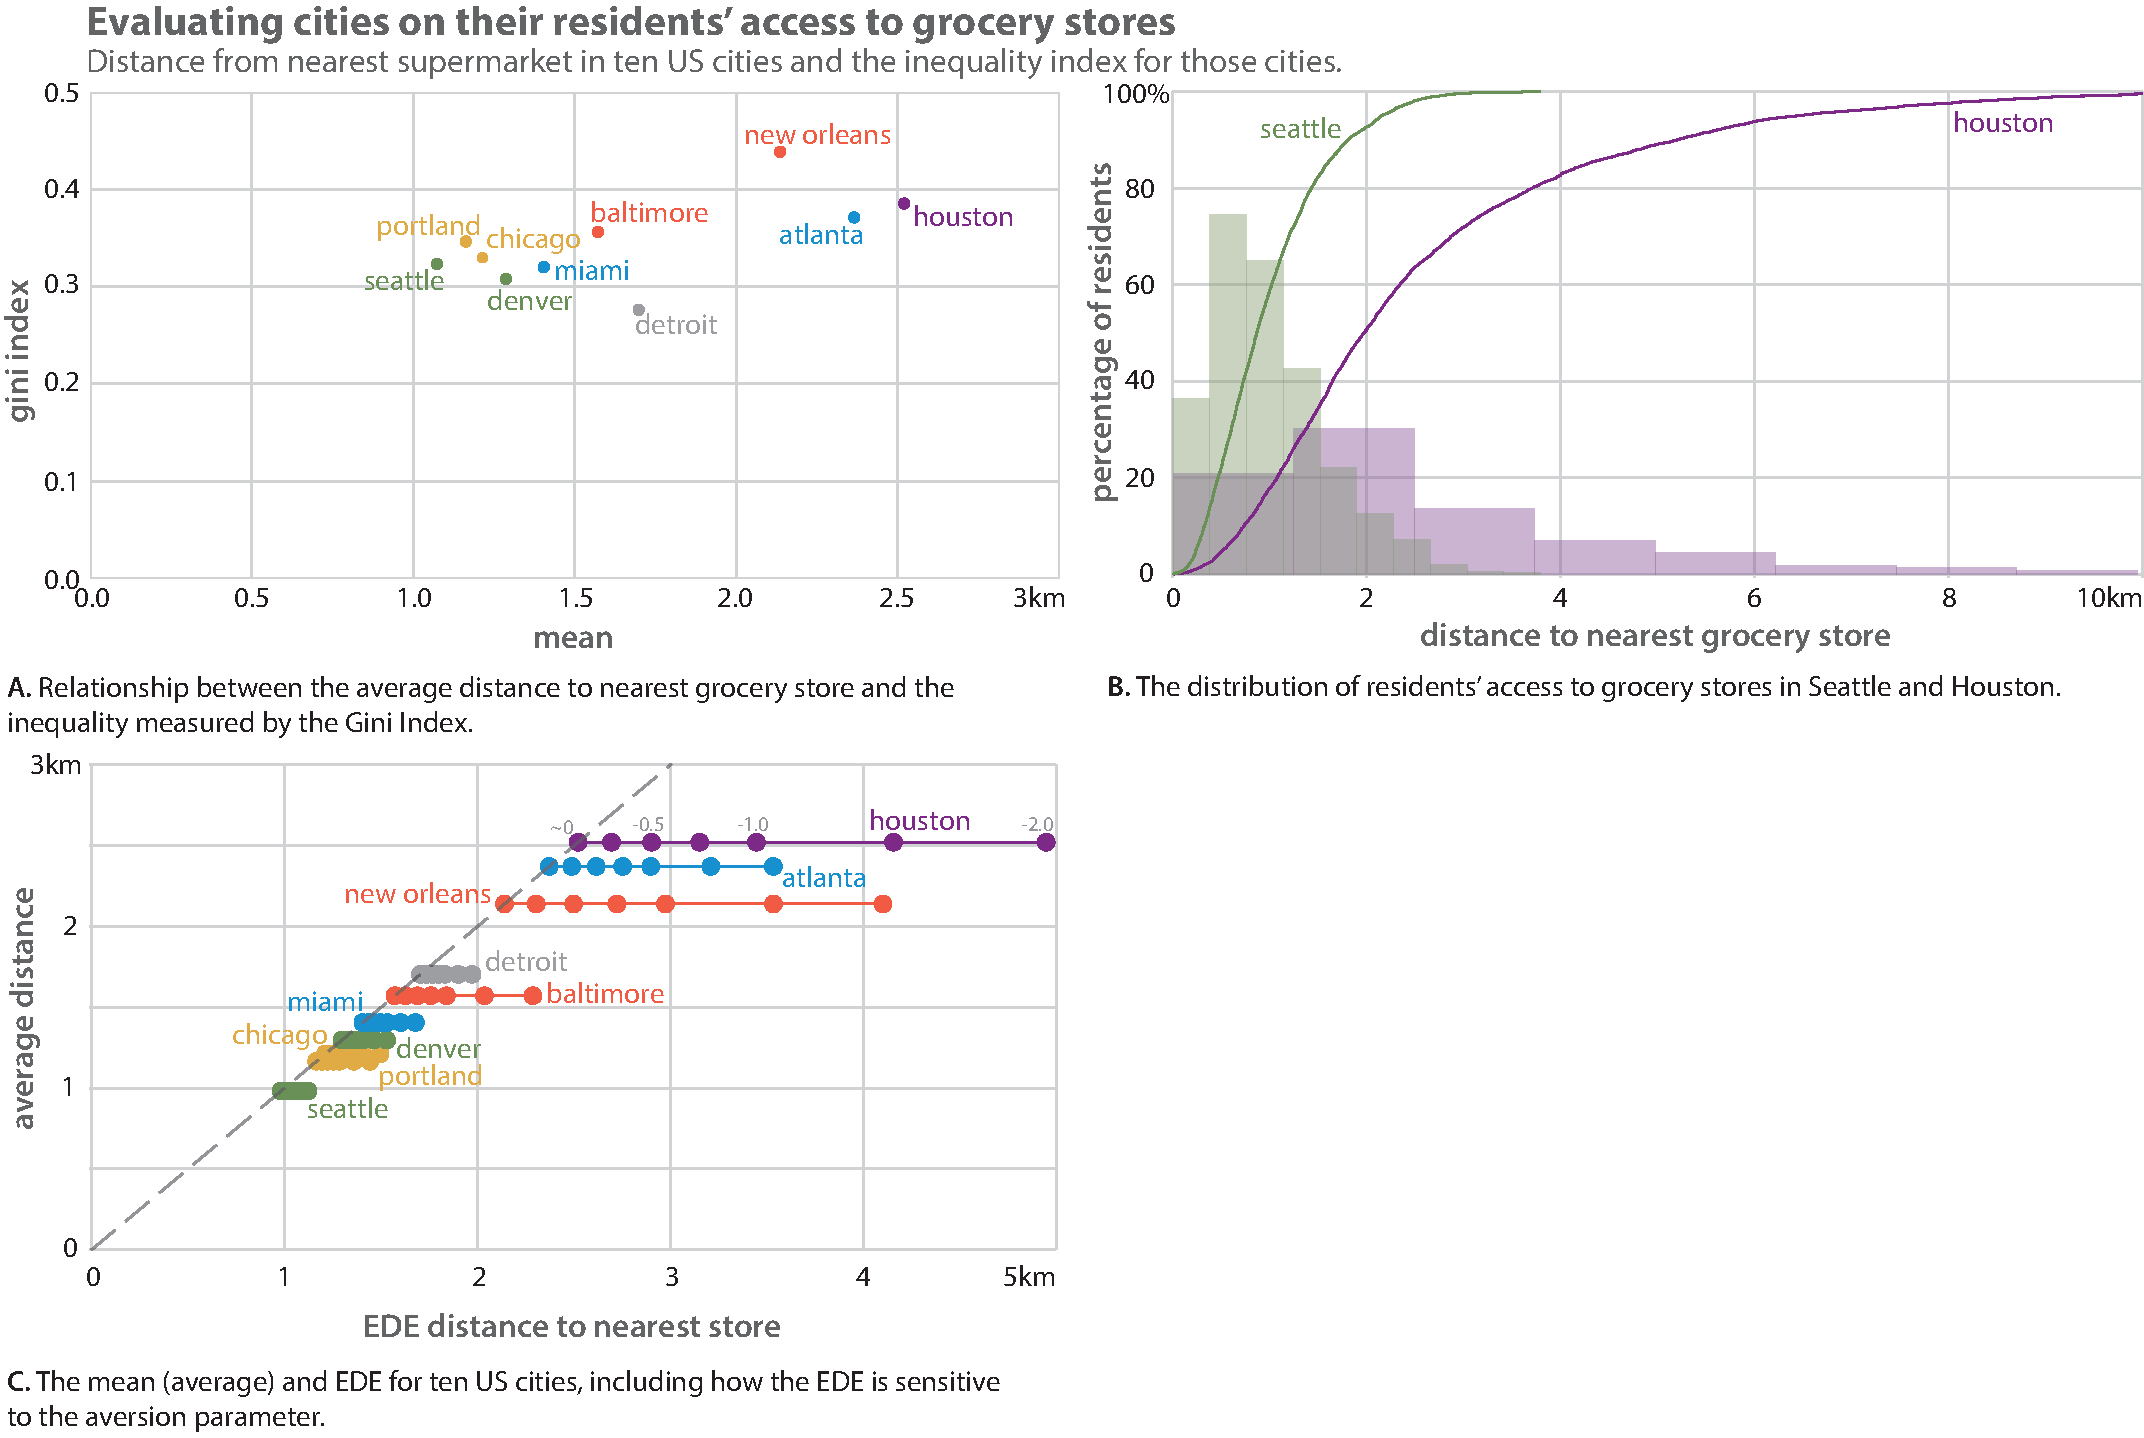
\includegraphics[width=\linewidth]{report/fig/fig2.pdf}
    \caption{
    Evaluating cities’ provision of grocery store access and the inequality in that access. In (C) we rank EDE and show how the EDE contrasts with the average value. By varying $\epsilon$ between $\sim$0 and 2 we observe how the aversion to inequality affects the EDE and the ranking between the cities.
    \label{fig:comparative}
    }
    
\end{figure*}

Our first case presents the comparative evaluation of access to grocery stores between ten cities in the USA.
We begin with a common approach to measuring inequality: the Gini Index.
Figure \ref{fig:comparative}A shows the Gini Index vs the average (mean) distance to the nearest store.
Such a figure is often used to represent both the location (absolute value) and relative dispersion (inequality) of a distribution (e.g., \cite{Adger1997-tu}).
It tells us approximately how good the access to grocery stores is in each of these ten cities as well as how that access is distributed, relatively, between the residents.
But which city has the better access to grocery stores?
Figure \ref{fig:comparative}B shows the distribution of residents' distance from grocery stores for both Seattle and Houston.
This figure shows that Seattle residents live much closer to grocery stores than those in Houston: on average, more than 1.5km closer. 
However, the Gini Index reports a similar level of inequality in Houston and Seattle.
Houston's Gini Index indicates it has a similar level of inequality to Portland and Baltimore as well.
The reason for this is that the Gini Index is scale-independent, so the wide variation in access for Houston's residents is normalized by the city's much larger average distance.
This scale-independence of the Gini Index is a limitation as it does not express that the experience for residents living in Seattle (for example) is much better than for residents living in Houston. 
While relative measures may be desirable in some contexts, such as when comparing wealth inequality between countries, it presents a major limitation in a planning context such as these.

This limitation is addressed by using the Kolm-Pollak EDE.
Figure \ref{fig:comparative}C presents a normative ordering of the cities, where the smaller the EDE, the better for people's access to grocery stores.
Seattle is the preferred city.
In this figure, we plot the EDE with a range of values for the aversion parameter ($\epsilon$).
When comparing different scenarios (or interventions in a decision-making context), exploring the sensitivity of preference/rank order to the parameter provides valuable information regarding our confidence in the preference or highlights the need to carefully agree on the aversion parameter's value (see Figure 7 in \cite{Atkinson1970-mr}).
In this case, Seattle is an exemplar for cities aiming to improve their access to grocery stores.
The EDE tells us that a value of $\sim$1km can be used to represent the access to grocery stores for all residents, accounting for inequality.

On the other hand, Houston is the worst city for grocery store access, of those studied.
Given a very low aversion to inequality, the EDE is greater than 2.5km to the nearest store (a food desert is often defined as 1.6km or further).
The EDE drastically increases as the aversion increases, reflective of the fact that many residents live more than 4km and even more than 8km (Figure \ref{fig:comparative}B) from a store.
This situation is poorly represented by the low Gini Index in Figure \ref{fig:comparative}A.

The importance of varying the aversion parameter is demonstrated by preference ordering between the cities of Atlanta and New Orleans in Figure \ref{fig:comparative}C.
Although Atlanta has a higher average distance to stores, as the aversion parameter increases, New Orleans moves from being 3rd to 2nd worst of the cities. 
This is due to New Orleans having wider disparities in access than Atlanta: that is, people with poor access in New Orleans are significantly farther from the nearest store (relative to those who are closest), compared with Atlanta residents with poor access; Baltimore also exhibits this issue.

To understand how the aversion parameter influences the Kolm-Pollak EDE, we assess the relationship in Figure~\ref{fig:aversion}.
Figure \ref{fig:aversion}A presents how the Kolm-Pollak EDE changes with $\epsilon$ (note that as $\kappa=f(\epsilon)$, see Equation \ref{eqn: kappa}, then $\Xi=f(\epsilon)$).
Although $\left|\epsilon\right|$ is traditionally varied between 0 and 2, we plot between 0 and 10 to better understand the behavior.
To understand this in the context of each distribution, \autoref{fig:aversion}B provides the distributions' percentiles.
When $\epsilon=0$ the EDE is equal to the expected value of the distribution.
As $\left|\epsilon\right| \rightarrow \infty$ the EDE trends to the maximum value of the distribution (i.e., the value of the worst-off individual).
Consider the lines of New Orleans, Atlanta, and Houston.
These three cities have relatively similar values for the average distance to the nearest store (between 2-2.5km) yet, the difference between these cities widens as the aversion to inequality parameter increases. 
As described before, the higher EDE as the aversion parameter increases is a reflection of New Orleans’s larger disparities as compared to Atlanta (compare their 75th and 90th percentiles).
Similarly, consider the case of Baltimore and Detroit.
Baltimore has a lower average distance than Detroit, but the residents at the 90th percentile in Baltimore are worse off than those at the 90th percentile in Detroit.
Again, the EDE reflects these disparities as the parameter for inequality aversion increases.
This shows the capability of this single metric to reflect both the average of a distribution as well as incorporate the state of the most disadvantaged people, often ignored by traditional metrics.

\begin{figure*}
    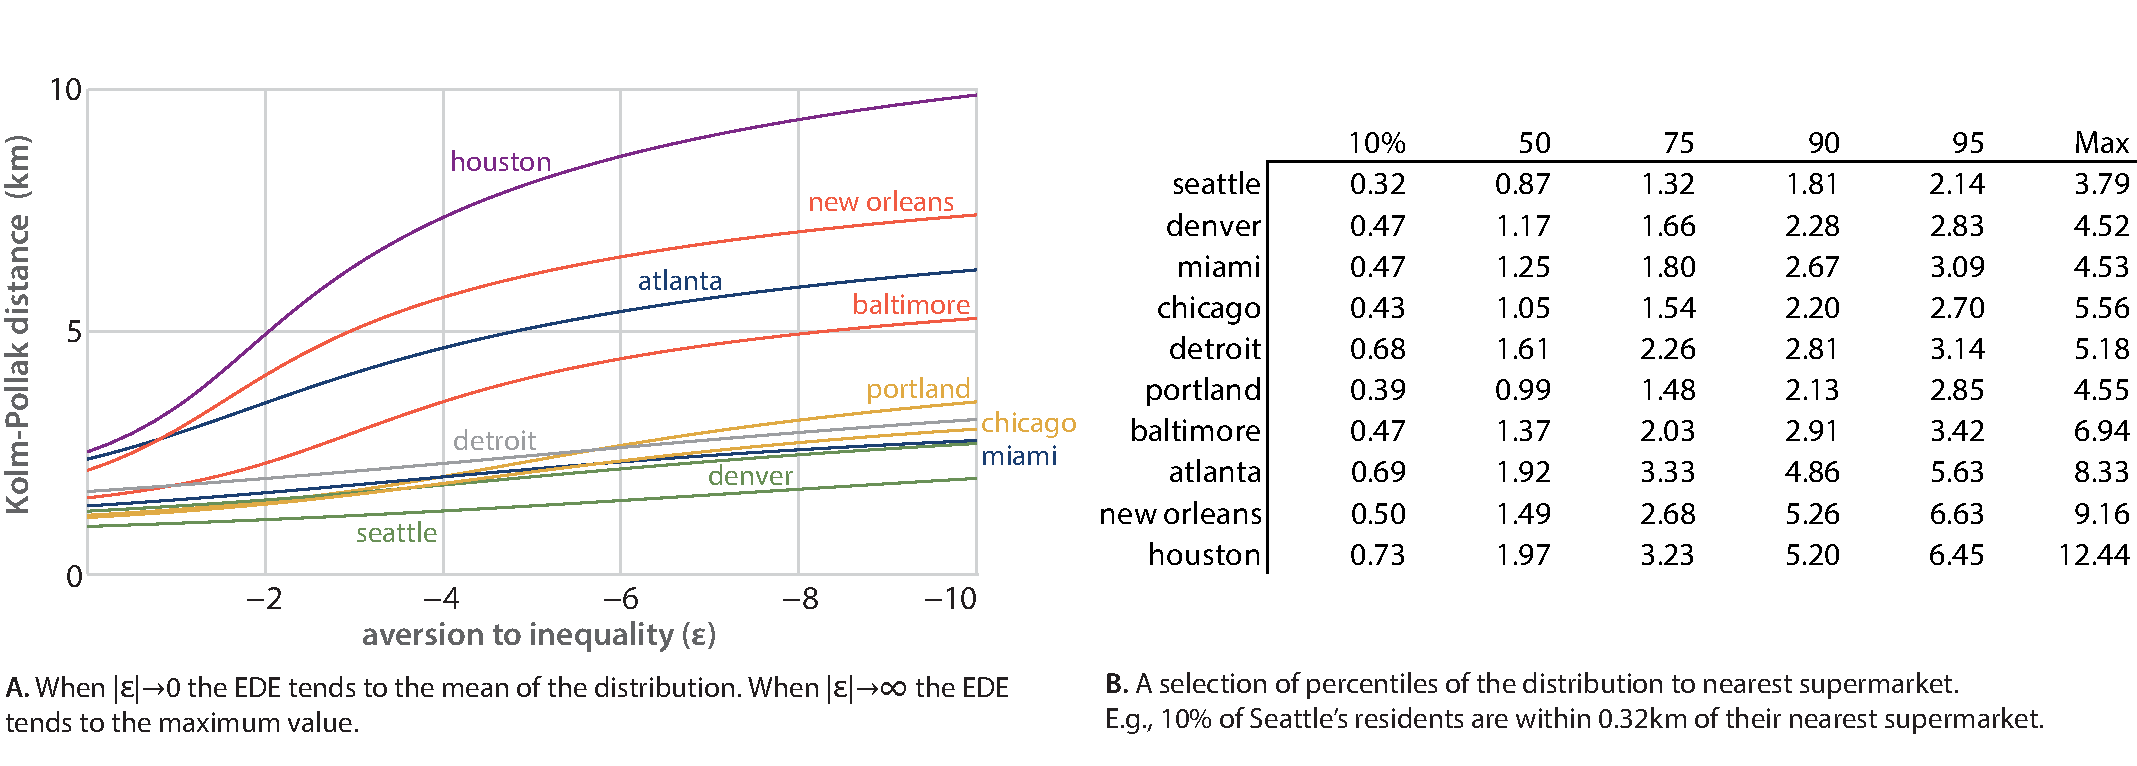
\includegraphics[width=\linewidth]{report/fig/fig3.pdf}
    \caption{
    Evaluating the sensitivity of the Kolm-Pollak EDE to changes in the aversion parameter. 
    }
    \label{fig:aversion}
\end{figure*}

\subsection{Comparing socio-economic subgroups}
To assess the equity of access we must consider the socioeconomic and demographic characteristics of the residents.
We evaluate the proximity to grocery stores in the ten cities for White residents, Black residents, and residents without vehicle access to demonstrate separability in the Kolm-Pollak method  (\autoref{fig:subgroup}; \autoref{tab:compare_demographics}).

In every city, Black residents have the same or worse access to grocery stores than residents in general, and this disparity is exacerbated when compared to White residents (Figure \ref{fig:subgroup}A).
Seattle and Portland have the distinction that there is no distinguishable difference between Black and White residents. 
Atlanta, New Orleans, and Houston have the widest disparity in access between racial groups.
Residents without vehicles have better access in five of the ten cities (including New Orleans) (Figure \ref{fig:subgroup}B).
However, in the remaining five cities including Atlanta, residents without cars have to travel further.
In eight of the ten cities, Black residents have an EDE of greater than 1.6km and in six of the ten cities, residents without access to a vehicle have an EDE higher than 1.6km. 
Given that 1 mile (1.6km) is the common measure for a food desert, and that our results overestimate access (because we include more stores than just supermarkets), this suggests there is limited healthy food access for these residents in the cities we examined.


\begin{figure*}
    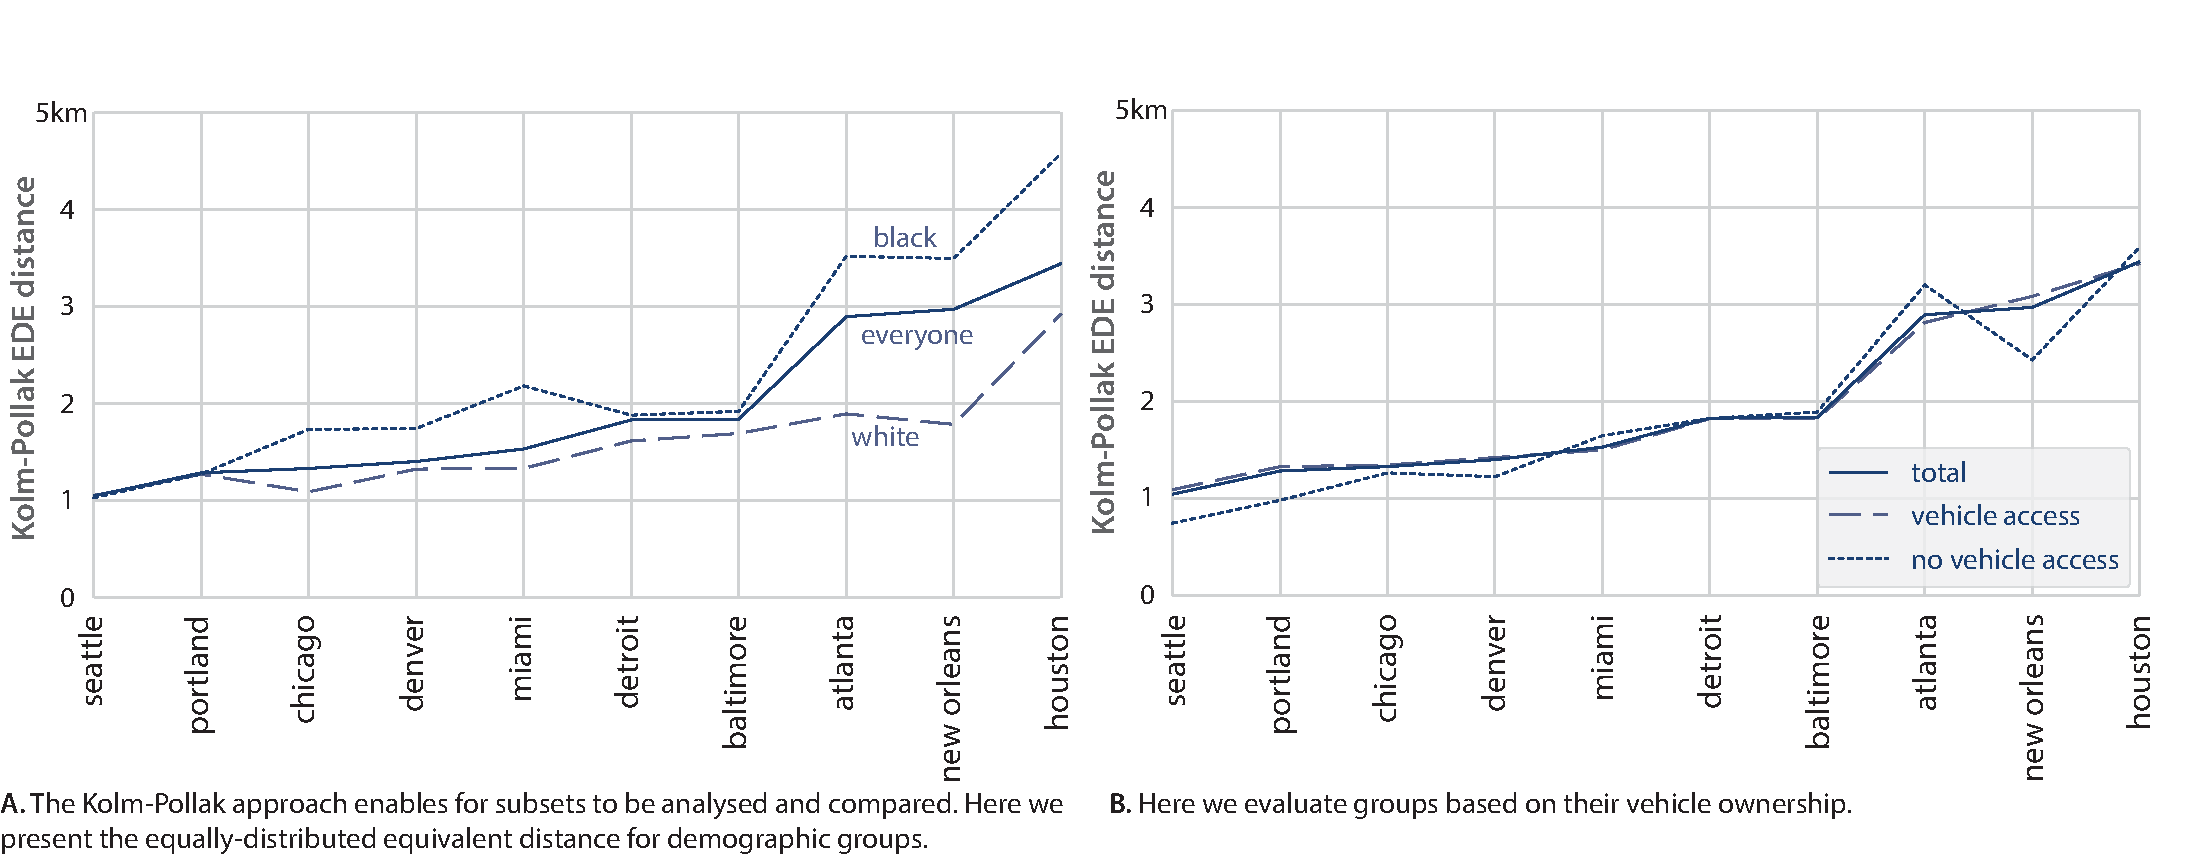
\includegraphics[width=\linewidth]{report/fig/fig4.pdf}
    \caption{
    Evaluating the proximity (penalized by inequality) of different demographic and socioeconomic groups to their nearest grocery store in ten USA cities. 
    An interactive plot is available at [redacted for review].
    }
    \label{fig:subgroup}
\end{figure*}

\begin{table}
\caption{The Kolm-Pollak EDE for the cities and demographic and socioeconomic subgroups}
\label{tab:compare_demographics}
\begin{tabular}{lrrrrrrrr}
\hline
\textbf{}   & \textbf{Total} & \textbf{White} & \textbf{Black} & \textbf{Am. Indian} & \textbf{Asian} & \textbf{Hisp/Latino} & \textbf{No vehicle} & \textbf{Poverty} \\ \hline
Atlanta     & 2.90           & 1.89           & 3.52           & 2.76                & 1.65           & 2.53                 & 3.21                & 3.24             \\
Baltimore   & 1.84           & 1.69           & 1.92           & 1.86                & 1.24           & 1.79                 & 1.89                & 1.92             \\
Chicago     & 1.33           & 1.09           & 1.73           & 1.23                & 0.96           & 1.22                 & 1.27                & 1.39             \\
Denver      & 1.40           & 1.32           & 1.74           & 1.36                & 1.44           & 1.47                 & 1.23                & 1.39             \\
Detroit     & 1.83           & 1.62           & 1.88           & 1.67                & 1.37           & 1.47                 & 1.83                & 1.86             \\
Houston     & 3.45           & 2.93           & 4.58           & 3.36                & 2.34           & 3.39                 & 3.59                & 3.78             \\
Miami       & 1.53           & 1.33           & 2.18           & 1.77                & 1.22           & 1.37                 & 1.65                & 1.68             \\
New Orleans & 2.97           & 1.79           & 3.50           & 2.39                & 2.71           & 2.22                 & 2.43                & 3.01             \\
Portland    & 1.29           & 1.27           & 1.27           & 1.21                & 1.46           & 1.28                 & 0.98                & 1.19             \\
Seattle     & 1.05           & 1.05           & 1.03           & 0.99                & 1.04           & 1.04                 & 0.75                & 0.87             \\ \hline
\end{tabular}
\end{table}

\subsection{Evaluating city-level planning scenarios}
In our final case, we investigate how access to \textit{supermarkets} has changed over time in Chicago.
This enables us to examine how planning decisions may have influenced the EDE over the past 13 years.
Chicago City has been actively working to improve access to healthy food \citep{cdph2012-si} and from 2011-2012 had secured commitments for new supermarkets in poorly served areas.
However, our timeline contains two notable events that set back this ambition:
the 2008 recession and Safeway closing all 14 of its supermarkets in 2013 \citep{Kolak2018-az}.

The year 2007 saw the best access to supermarkets for most subgroups within Chicago (Figure \ref{fig:chicago}).
By 2011, the situation had worsened for everyone except White and Asian residents, who in fact saw an improvement in supermarket access. 
Predictably, 2014 was the worst for all groups except Asians (who have seen consistently improving access and Hispanics and Latinos (whose access is deteriorating). 
As of 2020, the groups with improved access to supermarkets compared to 2007 are White and Asian residents, people with income below the poverty level, and people without access to vehicles.
Black residents have consistently had the worst access of all of the groups assessed.
Note, however, that our demographic and socioeconomic data are from the 2010 census and that our analysis only includes supermarkets using a specific, and relatively strict, definition to compare with the stores recorded in previous studies.
Nevertheless, this is further evidence of racial injustice despite improvement between 2014 and 2020.
% However, as the COVID-19 pandemic threatens another economic recession, significant and deliberate planning efforts will be necessary to ensure that store closures do not exacerbate disparities as they did between 2007 and 2011.
% Increased use of grocery delivery service to maintain isolation and support social distancing in the 2020 pandemic situation adds to the pressure on supermarkets;
% this could further stress vulnerable population groups who cannot afford online delivery and might experience growing inaccessibility due to store closures.

\begin{figure*}
    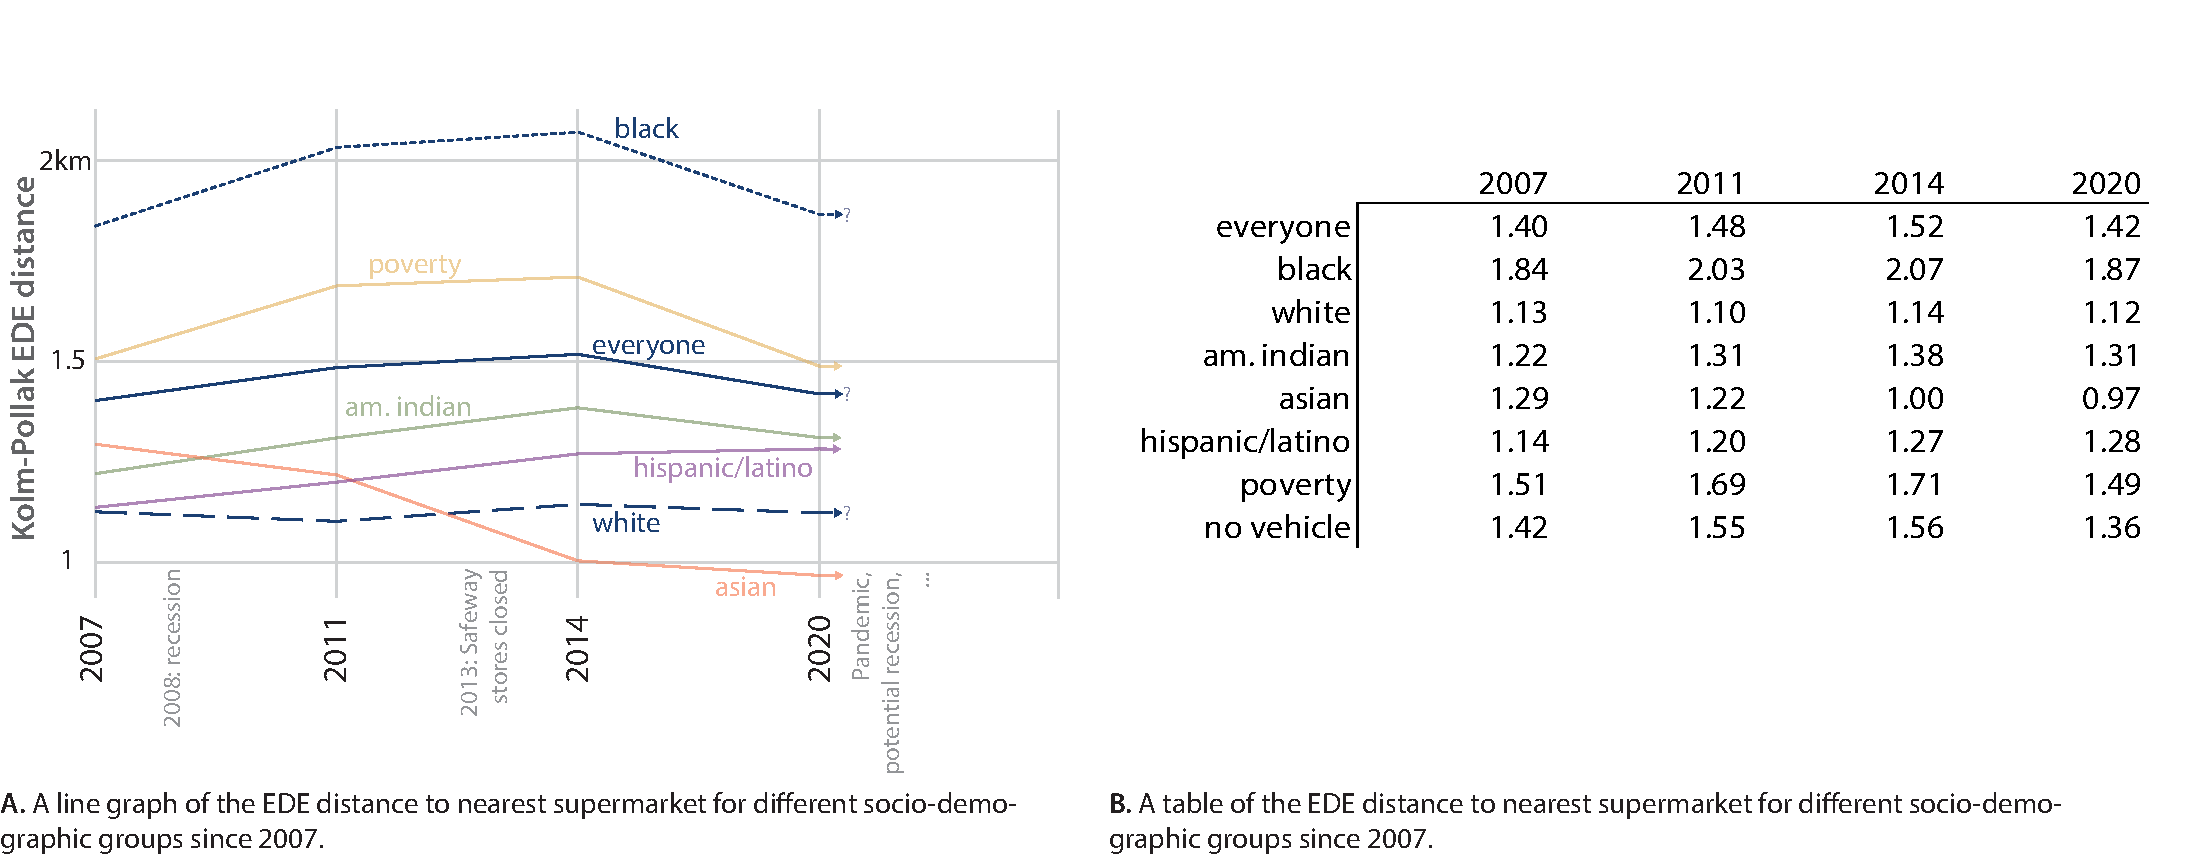
\includegraphics[width=\linewidth]{report/fig/fig5b.pdf}
    % \begin{subfigure}{0.5\textwidth}
    %     \includegraphics[width=0.9\linewidth]{report/fig/chicago_map_2014.pdf} 
    % \end{subfigure}
    % \begin{subfigure}{0.5\textwidth}
    %     \includegraphics[width=0.9\linewidth]{report/fig/chicago_map_2020.pdf}
    % \end{subfigure}
    \caption{
    How Chicago's access to supermarkets has changed over the past 13 years. 
    }
    \label{fig:chicago}
\end{figure*}

\section{Discussion and Conclusion}
\label{sec:discussion}
The ability to measure inequality in urban systems will enable planners to guide future urban development to promote equality and equity.
This is important for how we locate food resources and much more.
World-wide both amenities and burdens are inequitably distributed \citep{Fussel2010-te, Bulkeley2014-so} and it is essential that future development addresses these disparities \citep{Gusdorf2008-bm, Calvin2017-ja}.

We propose several criteria for an inequality measure for urban systems.
These criteria are generally similar to those proposed for an income inequality measure (\cite{Adger1997-tu, Blackwood1994-ie, Fields1978-tb}), but there are some important differences. 
Our proposed criteria are:
\begin{itemize}
    \item \textit{Symmetry}. Inequality of a population is based solely on the distribution of the quantity in question and no other rankings.
    \item \textit{Population independence}. The number of individuals does not influence the measure of inequality.
    \item \textit{Scale dependence}. The inequality measure should reflect the total sum of the quantity measured. For instance, high exposure to burdens (for example hazards or health risks) would be penalized.
    \item \textit{Principle of transfers}. If a quantity is redistributed from an advantaged individual to a disadvantaged individual, the inequality should decrease.
    \item Satisfies the \textit{mirror property.} The measure can be used for distributions of both desirable and undesirable quantities. 
    \item \textit{Separable.} The measure can be used to examine the inequality between subgroups (e.g., different demographic groups), and therefore can incorporate consideration of need or vulnerability, and, subsequently, inequity.
    \item \textit{Multivariate.} The measure can be used to evaluate multiple quantities and the correlation of (dis)advantages. 
\end{itemize}

The Kolm-Pollak EDE satisfies most of these criteria.
The case studies we explore in this paper, demonstrate the potential of the Kolm-Pollak approach to explore equality and equity of a quantity's distribution in urban systems.
We have shown how we can compare and rank several distributions, assess population subgroups, and compare scenarios across time, including how different socioeconomic/demographic groups fared given these changes.
That the Kolm-Pollak provides a metric combining both the distribution's location and dispersion is a significant advantage over traditional approaches (e.g., the Gini Index or ``percentage within a threshold'') by enabling distributions to be ranked based on both better access and lower inequality.
Traditional measures that suggest Seattle exhibits similar inequality than Houston are limited in a context where both preferences are considered simultaneously. 
We have also demonstrated the strength of the Kolm-Pollak approach in evaluating distributions of undesirable quantities (i.e., distance to an amenity where living closer is preferred over farther distances).
Existing measures are constructed for quantities where more is better (e.g., income).
Therefore, the Kolm-Pollak is useful for planners and others working in the built environment where negative or positive values may be relevant.

Within the context of spatial and mapping-based evaluations of equity, \cite{Kolak2018-az} note that measuring access in terms of citywide summary statistics of distance or number of opportunities is inadequate for illuminating disparities. 
LISA statistics may also fall short of fully quantifying equity, despite their utility in determining where significant spatial patterns are located. 
Results from LISA-based analyses locate problematic clusters or outliers, indicating inequality in relationships between variables in neighboring areas. 
However, demonstrating where spatial inequality is present does not directly measure inequity because meeting the unique needs of some residents may require spatial inequality in how a resource or quantity is distributed.
Where LISA’s global counterparts only provide a single summary value indicating whether clusters are present and summary statistics of spatial metrics are insufficient, the Kolm-Pollak approach supplements spatial pattern perspectives by quantifying the degree to which inequality is problematic at broader (e.g., citywide) scales and among population subgroups. 
Applied together, these measures suitably evaluate inequality as well as the locational clustering of individual values that may contribute to that inequality.

The Kolm-Pollak measure provides a way to quantify the performance and inequality of a quantity's distribution within the built environment.
It enables inequality assessment to become the ``new normal'' and a primary consideration when evaluating interventions and general long-term planning. 
Its use does not require a change in the analysis method; it simply replaces previous metrics such as the average or `percentage within a threshold.'
This presents numerous opportunities for planners, especially with the growing interest in data-driven planning, as it enables us to evaluate the distribution of desirable and undesirable quantities and to compare between subgroups.
While map-based visualizations are irreplaceable and will always be necessary for communicating the spatial distribution of quantities throughout a region, the EDE can be used in quantitative analysis for ranking or optimization that support decision-making, while capturing inequality.
For example, where previous studies have used thresholds (e.g., ParkScore's percentage of people within a 10-minute walk to their nearest green space) or summary statistics in regression-type analysis, the EDE can enhance these same analyses to factor in inequality.

As we described earlier, the primary limitation of the Kolm-Pollak EDE and associated inequality index is that it measures a single quantity.
However, where \cite{Cox2012-lg} criticizes inequality measures for their potential to overstate inequality (arguing that the inequality of being exposed to more pollution is compensated for by lower house prices), we raise the more insidious potential that we may underestimate the injustices.
The EDE approach can only be used to evaluate a single quantity and enables us to discuss inequity in (e.g.,) supermarket access, but the challenge remains as to how we assess multivariate and potentially compounding burdens.
For example, poverty and lack of supermarket access, or poverty, lack of supermarket access, and lack of recreational opportunities may be exacerbated by the intersectionality of these factors.
In air quality examinations (the subject of \cite{Cox2012-lg}'s criticism), this approach does not enable us to evaluate the health risk of complex mixtures of chemicals, for example, which highlights the importance of evaluating the distributions of environmental injustice and how we must take pains to not \textit{underestimate} these burdens or inequities.

The ability to evaluate equality and ensure equity will be increasingly important as our cities continue to change over the next few years and decades.
The economic crash that may emerge from the pandemic could have widespread negative impacts on vulnerable communities, many of which have already faced inequality with increased exposure risks \citep{patel2020-poverty} and reduced resource access \citep{power2020-covid}. 
Beyond access to supermarkets, lack of funding may produce or exacerbate barriers to other resources and protective opportunities such as employment, health care, and safe green space for physical activity, as decision-makers navigate fiscal constraints.
This is likely compounded further as the current leadership slashes environmental protections and threatens to add to the burdens on water, air, and noise quality.

While the pandemic and climate change both present threats, there is also the opportunity to vastly improve our cities given the investments by governments worldwide to restart economies.
The Kolm-Pollak method enables cities to set and evaluate targets on urban characteristics, including but not limited to access to essential services. 
Policy and planning to address food-deserts and other service-deserts could foster improved, equitable access to these services, thus reducing carbon emissions and improving community resilience.
As demonstrated in our case studies, the Kolm-Pollak EDE is invaluable in equipping planners and decision-makers with the evidence needed when advocating for accessible, sustainable, and just societies.

\section{Acknowledgments}
% MJA was funded by the Department of Civil and Natural Resources Engineering at the University of Canterbury, this support is much appreciated.

\bibliography{mybibfile}



\end{document}

